\chapter{Assunzioni e Ipotesi}
\label{ch:assunzioni}
Dalle prime analisi effettuate sul dataset si sono riscontrati alcuni problemi rispetto alla gestione delle classi di qualità.

\noindent
Come già descritto in precedenza, sono presenti ben 10 differenti classi di qualità tra vini rossi e vini bianchi e questo porta a dover gestire un problema di classificazione a 10 classi.

\noindent
Dopo aver osservato tramite l'analisi del dataset le varie distribuzioni dei dati si è scelto di raggruppare le classi di qualità riconducendosi a un problema di classificazione binaria.

\noindent
In questo capitolo vengono mostrati i grafici e spiegate le motivazioni che hanno portato questa scelta.

\begin{itemize}
    \item \textbf{Classificazione a 10 classi}: ovvero quella originale rappresentata nel dataset.
    \item \textbf{Classificazione a 2 classi}: raggruppando le classi originali in modo tale che i vini di qualità inferiore alla qualità originale 6 compresa sono vini di bassa qualità mentre i restanti fanno parte dei vini di alta qualità.
\end{itemize}

\noindent
Le due tipologie sono state confrontate per poter scegliere quale risultasse la migliore. In primo luogo sono state osservate le distribuzioni rispetto al numero di istanze [\ref{fig:quality_different_class}].

\newpage

\begin{figure}[H]
    \centering
    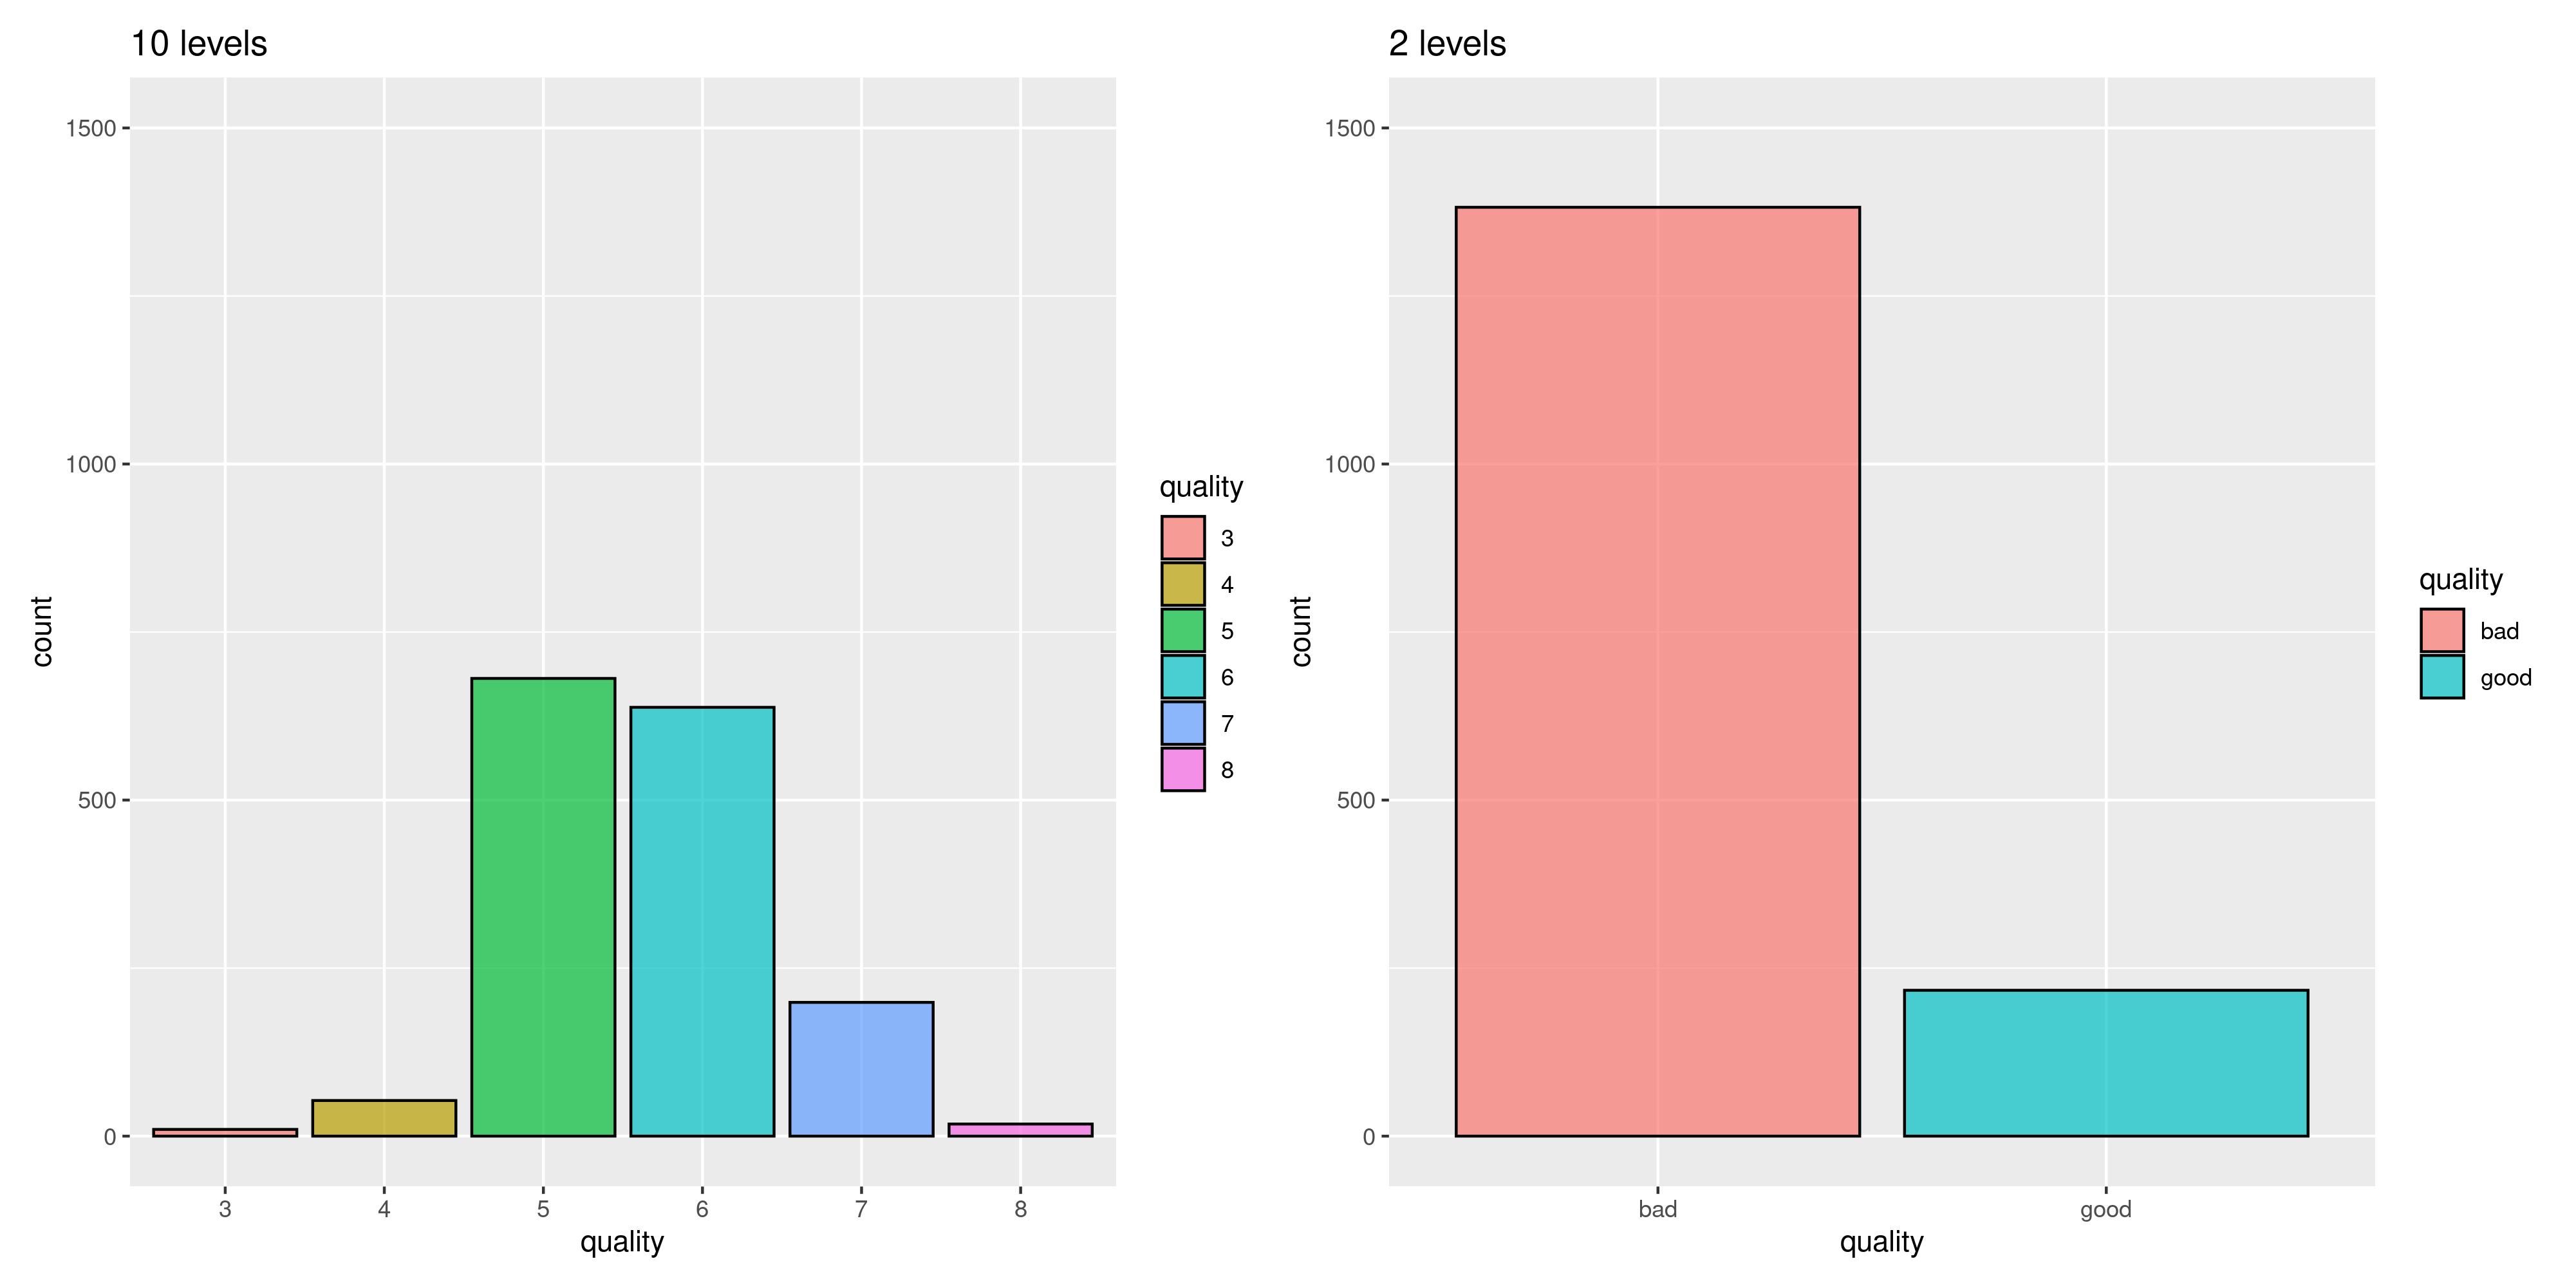
\includegraphics[width=\textwidth]{images/analisi/class_hist_binary.png}
    \caption{grafico che rappresenta la distribuzione dei dati rispetto alle due tipologie di classificazione prese in considerazione}
    \label{fig:quality_different_class}
\end{figure}

\noindent
Da questa analisi si è notato come le istanze non siano distribuite in modo uniforme, anzi si ha una prevalenza di dati rispetto alle qualità centrali e una scarsa rappresentazione delle qualità più basse e più alte, per questo motivo si è scartata l'ipotesi di poter sfruttare una classificazione a 10 classi, perché non in grado di rappresentare in modo appropriato le 10 classi.

\noindent
Osservando il grafico [\ref{fig:quality_different_class}] si può notare come per alcune classi di qualità non siano presenti istanze che li rappresentino.

\noindent
La classificazione a due classi è stata scelta perché anche se sbilanciata ha un buon numero di istanze che rappresentano sia la qualità bassa sia la qualità alta.

\noindent
Inoltre si è scelto di operare solamente usando una tipologia di vino perché operare considerando contemporaneamente vini bianchi e vini rossi rende più complessa la distinzione tra vini di bassa e alta qualità, questo per via delle loro diverse caratteristiche fisico-chimiche che li contraddistinguono.

\noindent
Quindi è stata considerata solamente la porzione di dataset relativa ai vini rossi, analogamente lo stesso procedimento può essere implementato per i vini bianchi. 